%% vim:tw=66:spell:wrap:ft=tex
\documentclass[%
        hyperref={%
                pdfauthor={Zakariyya Mughal},%
                pdfpagemode={None},pdfpagelayout={SinglePage}}%
        xcolor={x11names},%
]{beamer}
\usetheme{Warsaw}
\usecolortheme{crane}
\usepackage{textcomp}
\usepackage{fancyvrb}
\usepackage{changepage}
\usepackage{multicol}
\usepackage{wasysym}
\newenvironment{indented}{\begin{adjustwidth}{1.5em}{}}{\end{adjustwidth}}

\title[Git/GitHub]{Learning to use Git and GitHub to collaborate $\heartsuit$}
\author{Zaki Mughal}
\institute{University of Houston:\\CougarCS}
\date{2013 Feb 14}
\begin{document}

\frame{\titlepage}

\begin{frame}
\frametitle{Intro}
\begin{center}
\Huge
What is Git?
\end{center}
\end{frame}

\begin{frame}
\frametitle{Intro}
\begin{itemize}
\item[] It's version control
\pause \item[] What?
\end{itemize}
\end{frame}

\begin{frame}
\frametitle{Intro}
\begin{itemize}
\item[] Suppose you're working on code
\pause \item[] make some changes
\pause \item[] \qquad still works
\pause \item[] make some changes
\pause \item[] \qquad still works
\pause \item[] make some changes
\pause \item[] \qquad broken?!
\end{itemize}
\end{frame}

\begin{frame}
\frametitle{Intro}

\includegraphics[width=\textwidth]{gfx/no-idea.jpg}
\end{frame}

\begin{frame}
\frametitle{Intro}
\begin{itemize}
\item[] Broken?
\pause \item[] \qquad but where?
\pause \item[] \qquad \qquad start /* commenting */ things out
\pause \item[] \qquad \qquad \qquad you start to lose your mind
\end{itemize}
\end{frame}

\begin{frame}
\frametitle{Intro}
\begin{center}

\includegraphics[height=0.85\textheight]{gfx/wat.jpg}
\end{center}
\end{frame}

\begin{frame}
\frametitle{Intro}
\begin{center}
\Huge
Do not want.
\end{center}
\end{frame}

\begin{frame}
\frametitle{Intro}
\begin{itemize}
\item[] Sharing code
\pause \item[] \qquad somebody wants a copy of your code
\pause \item[] \qquad \qquad they make changes to their copy
\pause \item[] \qquad \qquad you make changes to your copy
\pause \item[] \qquad \qquad AT THE SAME TIME
\pause \item[] \qquad Now you want to share the changes with each other
\pause \item[] \qquad \qquad \ldots
\pause \item[] \qquad \qquad \ldots merging?
\end{itemize}
\end{frame}

\begin{frame}
\frametitle{Intro}

\includegraphics[width=\textwidth]{gfx/nonono.png}
\end{frame}

\begin{frame}
\frametitle{Intro}
\begin{itemize}
\item[] Ever seen a project folder like:
\item[] \qquad \texttt{main.c}
\item[] \qquad \texttt{main.c.old}
\item[] \qquad \texttt{main.c.fixed}
\item[] \qquad \texttt{main.c.actually\_fixed}
\item[] \qquad \texttt{main.c.this\_one\_really}
\item[] \qquad \texttt{main.c.final}
\end{itemize}
\end{frame}

\begin{frame}
\frametitle{Intro}
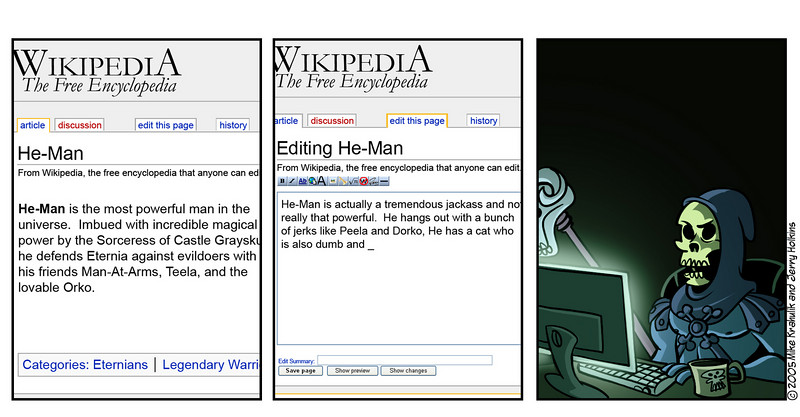
\includegraphics[width=\textwidth]{gfx/skeletor.jpg}
\end{frame}

\begin{frame}
\frametitle{Intro}
\begin{itemize}
	\item [] Wikipedia's page history
	\pause \item [] \texttt{diff} (Unix tool)
	\pause \item [] \href{https://en.wikipedia.org/wiki/Longest_common_subsequence_problem}{Longest common subsequence problem}
\end{itemize}
\end{frame}

\begin{frame}
\frametitle{Intro}
Basics of version control
\begin{itemize}
	\item [] fetch a specific version of a file
	\pause \item [] store the changes to relative to a specific version of a file
\end{itemize}
\end{frame}

\begin{frame}
\frametitle{Intro}
\begin{itemize}
	\item [] Lots of version control software exists
	\pause \item []\qquad CVS, Subversion, Team Foundation Server, Perforce
	\pause \item []\qquad\qquad client-server model
	\pause \item []\qquad\qquad you need a network
\end{itemize}
\end{frame}

\begin{frame}
\frametitle{Intro}

\includegraphics[width=\textwidth]{gfx/laptop-beach.jpg}
\end{frame}

\begin{frame}
\frametitle{Intro}
\begin{itemize}
	\item [] Git is distributed
	\pause \item []\qquad all commands are done locally
	\pause \item []\qquad\qquad each copy contains all older versions
	\pause \item []\qquad developed by Linus Torvalds for
		Linux kernel development
	\pause \item []\qquad\qquad need for fast branching/merging
	\item []\qquad\qquad	(more on this in a bit)
\end{itemize}
\end{frame}

\begin{frame}
\frametitle{Get on with (g)it!}
\begin{center}
\Huge
$<$\href{http://try.github.com/}{http://try.github.com/}$>$
\end{center}
\end{frame}

\begin{frame}
\frametitle{Installing git}
\begin{itemize}
	\item []Debian/Ubuntu
	\item[]\qquad apt-get install git
	\pause \item[]Windows
	\item[]\qquad $<$\href{http://msysgit.github.com/}{http://msysgit.github.com/}$>$
\end{itemize}
\end{frame}

\begin{frame}[fragile]
\frametitle{Setting it up}
\begin{verbatim}
	git config --global user.name "Batman"
	git config --global user.email "batman@jl.org"
\end{verbatim}
\end{frame}

\begin{frame}
\frametitle{Setting it up $>\_>$}
\begin{center}

\includegraphics[height=0.9\textheight]{gfx/smbc-batman.png}
\end{center}
\end{frame}

\begin{frame}
\begin{center}
	\Huge Upload slides
\end{center}
\end{frame}

\begin{frame}
\frametitle{GitHub clients (more graphical)}
\begin{itemize}
	\item[] $<$\href{http://eclipse.github.com/}{http://eclipse.github.com/}$>$
	\item[] $<$\href{http://mac.github.com/}{http://mac.github.com/}$>$
	\item[] $<$\href{http://windows.github.com/}{http://windows.github.com/}$>$
\end{itemize}
\end{frame}

\begin{frame}[allowframebreaks]
	\frametitle{Why upload and contribute your code?}
		\begin{itemize}
		\item[] improve your skills
			\begin{description}
				\item[] reading good books makes you a better writer
				\item[] reading good code makes you a better coder
			\end{description}
		\item[] show your skills
			\begin{description}
				\item[] many tech-oriented companies will look for your code online
				\item[] \qquad {\Large portfolio}
				\item[] at a job interview: ``I
					helped write some of the
					code you use daily''
			\end{description}
		\framebreak
		\item[] collaborate with others all around the world
			\begin{description}
				\item[] you may not share the same mother tongue, but you can both speak with code
				\item[] programming in the large
				\item[] \qquad how code is managed in projects
			\end{description}
		\item[] don't have enough skills yet?
			\begin{description}
				\item[] you can lend a hand in other ways
				\item[] \qquad graphic design\ldots
				\item[] \qquad documentation\ldots
				\item[] $<$\href{http://open-advice.org/}{http://open-advice.org/}$>$
			\end{description}
		\end{itemize}
\end{frame}

\begin{frame}
\frametitle{Learn more?}
\begin{description}
\item[Pro Git book]
	$<$\href{http://git-scm.com/book}{http://git-scm.com/book}$>$
\item[man pages (reference)]
	$<$\href{http://git-scm.com/docs}{http://git-scm.com/docs}$>$
\item[IRC: \#git on freenode]
	$<$\href{http://jk.gs/git/}{http://jk.gs/git/}$>$
\item[git for computer scientists]
	$<$\href{http://eagain.net/articles/git-for-computer-scientists/}{http://eagain.net/articles/git-for-computer-scientists/}$>$
\item[git concepts simplified]
	$<$\href{http://sitaramc.github.com/gcs/}{http://sitaramc.github.com/gcs/}$>$
\end{description}
\end{frame}

\end{document}
